%-------------------------------------
% LaTeX Resume for Software Engineers
% Author : Leslie Cheng
% License : MIT
%-------------------------------------

\documentclass[letterpaper,12pt]{article}[leftmargin=*]

\usepackage[empty]{fullpage}
\usepackage{enumitem}
\usepackage{ifxetex}
\ifxetex
  \usepackage{fontspec}
  \usepackage[xetex]{hyperref}
\else
  \usepackage[utf8]{inputenc}
  \usepackage[T1]{fontenc}
  \usepackage[pdftex]{hyperref}
\fi
\usepackage{fontawesome}
\usepackage[sfdefault,light]{FiraSans}
\usepackage{anyfontsize}
\usepackage{xcolor}
\usepackage{tabularx}

\usepackage{graphicx}


%-------------------------------------------------- SETTINGS HERE --------------------------------------------------
% Header settings
\def \fullname {Zheren Huang}
\def \subtitle {}

\def \linkedinicon {\faLinkedin}
\def \linkedinlink {https://linkedin.com/in/zheren-huang-9133a6235/}
\def \linkedintext {linkedin.com/in/zheren-huang}

\def \phoneicon {\faPhone}
\def \phonetext {+61 466641756}

\def \emailicon {\faEnvelope}
\def \emaillink {mailto:zherenh@outlook.com}
\def \emailtext {zherenh@outlook.com}

\def \githubicon {\faGithub}
\def \githublink {https://github.com/1diotprogrammer}
\def \githubtext {zherenh-1diotprogrammer}

\def \websiteicon {\faGlobe}
\def \websitelink {https://blog.csdn.net/ooooobx?spm=1000.2115.3001.5343}
\def \websitetext {zherenh-CSDN.com}

\def \headertype {\doublecol} % \singlecol or \doublecol

% Misc settings
\def \entryspacing {-0pt}

\def \bulletstyle {\faAngleRight}

% Define colours
\definecolor{primary}{HTML}{000000}
\definecolor{secondary}{HTML}{0D47A1}
\definecolor{accent}{HTML}{263238}
\definecolor{links}{HTML}{1565C0}

%------------------------------------------------------------------------------------------------------------------- 

% Defines to make listing easier
\def \linkedin {\linkedinicon \hspace{3pt}\href{\linkedinlink}{\linkedintext}}
\def \phone {\phoneicon \hspace{3pt}{ \phonetext}}
\def \email {\emailicon \hspace{3pt}\href{\emaillink}{\emailtext}}
\def \github {\githubicon \hspace{3pt}\href{\githublink}{\githubtext}}
\def \website {\websiteicon \hspace{3pt}\href{\websitelink}{\websitetext}}

% Adjust margins
\addtolength{\oddsidemargin}{-0.55in}
\addtolength{\evensidemargin}{-0.55in}
\addtolength{\textwidth}{1.1in}
\addtolength{\topmargin}{-0.6in}
\addtolength{\textheight}{1.1in}

% Define the link colours
\hypersetup{
    colorlinks=true,
    urlcolor=links,
}

% Set the margin alignment 
\raggedbottom
\raggedright
\setlength{\tabcolsep}{0in}

%-------------------------
% Custom commands

% Sections
\renewcommand{\section}[2]{\vspace{5pt}
  \colorbox{secondary}{\color{white}\raggedbottom\normalsize\textbf{{#1}{\hspace{7pt}#2}}}
}

% Entry start and end, for spacing
\newcommand{\resumeEntryStart}{\begin{itemize}[leftmargin=2.5mm]}
\newcommand{\resumeEntryEnd}{\end{itemize}\vspace{\entryspacing}}

% Itemized list for the bullet points under an entry, if necessary
\newcommand{\resumeItemListStart}{\begin{itemize}[leftmargin=4.5mm]}
\newcommand{\resumeItemListEnd}{\end{itemize}}

% Resume item
\renewcommand{\labelitemii}{\bulletstyle}
\newcommand{\resumeItem}[1]{
  \item\small{
    {#1 \vspace{-2pt}}
  }
}

% Entry with title, subheading, date(s), and location
\newcommand{\resumeEntryTSDL}[4]{
  \vspace{-1pt}\item[]
    \begin{tabularx}{0.97\textwidth}{X@{\hspace{60pt}}r}
      \textbf{\color{primary}#1} & {\firabook\color{accent}\small#2} \\
      \textit{\color{accent}\small#3} & \textit{\color{accent}\small#4} \\
    \end{tabularx}\vspace{-6pt}
}

% Entry with title and date(s)
\newcommand{\resumeEntryTD}[2]{
  \vspace{-1pt}\item[]
    \begin{tabularx}{0.97\textwidth}{X@{\hspace{60pt}}r}
      \textbf{\color{primary}#1} & {\firabook\color{accent}\small#2} \\
    \end{tabularx}\vspace{-6pt}
}

% Entry for special (skills)
\newcommand{\resumeEntryS}[2]{
  \item[]\small{
    \textbf{\color{primary}#1 }{ #2 \vspace{-6pt}}
  }
}

% Double column header
\newcommand{\doublecol}[6]{
  \begin{tabularx}{\textwidth}{Xr}
    {
      \begin{tabular}[c]{l}
        \fontsize{35}{45}\selectfont{\color{primary}{{\textbf{\fullname}}}} \\
        {\textit{\subtitle}} % You could add a subtitle here
      \end{tabular}
    } & {
      \begin{tabular}[c]{l@{\hspace{1.5em}}l}
        {\small#4} & {\small#1} \\
        {\small#5} & {\small#2} \\
        {\small#6} & {\small#3}
      \end{tabular}
    }
  \end{tabularx}
}

% Single column header
\newcommand{\singlecol}[6]{
  \begin{tabularx}{\textwidth}{Xr}
    {
      \begin{tabular}[b]{l}
        \fontsize{35}{45}\selectfont{\color{primary}{{\textbf{\fullname}}}} \\
        {\textit{\subtitle}} % You could add a subtitle here
      \end{tabular}
    } & {
      \begin{tabular}[c]{l}
        {\small#1} \\
        {\small#2} \\
        {\small#3} \\
        {\small#4} \\
        {\small#5} \\
        {\small#6}
      \end{tabular}
    }
  \end{tabularx}
}

\begin{document}
%-------------------------------------------------- BEGIN HERE --------------------------------------------------

%---------------------------------------------------- HEADER ----------------------------------------------------

\headertype{\linkedin}{\github}{\website}{\phone}{\email}{} % Set the order of items here
\vspace{-10pt} % Set a negative value to push the body up, and the opposite

%-------------------------------------------------- EDUCATION --------------------------------------------------
  \resumeEntryStart
  \resumeEntryEnd
  \resumeEntryStart
  \resumeEntryEnd

  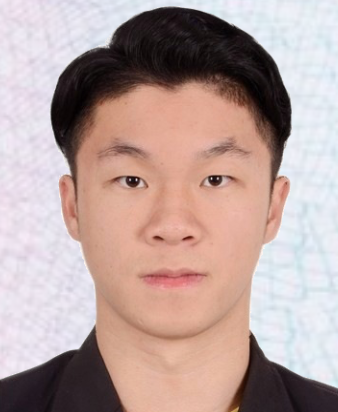
\includegraphics[scale=0.4]{IDPhoto.jpg}

\section{\faGraduationCap}{Education}

  \resumeEntryStart
    \resumeEntryTSDL
      {University Of Melbourne}{2020 -- 2022}
      {CS Computer Science and Software, wam 75}{Melbourne, VIC}
  \resumeEntryEnd
  
  \resumeEntryStart
    \resumeEntryTSDL
      {Dulwich International High School}{2015 -- 2019}
      {A-Level FurtherMath A*}{Zhuhai, Guangdong}
  \resumeEntryEnd
  
  \resumeEntryStart
    \resumeEntryEnd

%-------------------------------------------------- EXPERIENCE --------------------------------------------------
\section{\faPieChart}{Experience}

  \resumeEntryStart
    \resumeEntryTSDL
      {King Soft}{Nov. 2021 -- Feb. 2022}
      {Software Developer Internship}{Zhuhai, Guangdong}
    \resumeItemListStart
      \resumeItem {Writing the cross-platform ini configuration files}
      \resumeItem {Setting the structure of multithreading and database}
      \resumeItem {Complete the coding about some Application Virtualization operation}
    \resumeItemListEnd
  \resumeEntryEnd
  
  \resumeEntryStart
  \resumeEntryEnd

%-------------------------------------------------- PROJECTS --------------------------------------------------
\section{\faFlask}{Projects}

  \resumeEntryStart
    \resumeEntryTD
      {JX3 and JX3Client}{}
    \resumeItemListStart
      \resumeItem {Not in the core development team, but participating the ini configuration files coding.}
    \resumeItemListEnd
  \resumeEntryEnd

  \resumeEntryStart
    \resumeEntryTD
      {Diabete@Home}{}
    \resumeItemListStart
      \resumeItem {A website app about the patient data recording which still under development.}
    \resumeItemListEnd
  \resumeEntryEnd
  
  \resumeEntryStart
  \resumeEntryEnd

%-------------------------------------------------- PROGRAMMING SKILLS --------------------------------------------------
\section{\faGears}{Skills}
 \resumeEntryStart
  \resumeEntryS{Basic } {Proficient in front-end CSS/JS, Know well C++ Language, Comprehend web app frame including react, express, heroku, MySQL and MongoDB}
  \resumeEntryS{Traits } {Hardworking, Willing working extra hours, Outgoing, Good communicators, Interested in front-end positions}
 \resumeEntryEnd

\end{document}
